\section{The ranking of the optimizers flips with the horizon}
\label{sec:interaction}

\begin{figure*}[t]
\centering
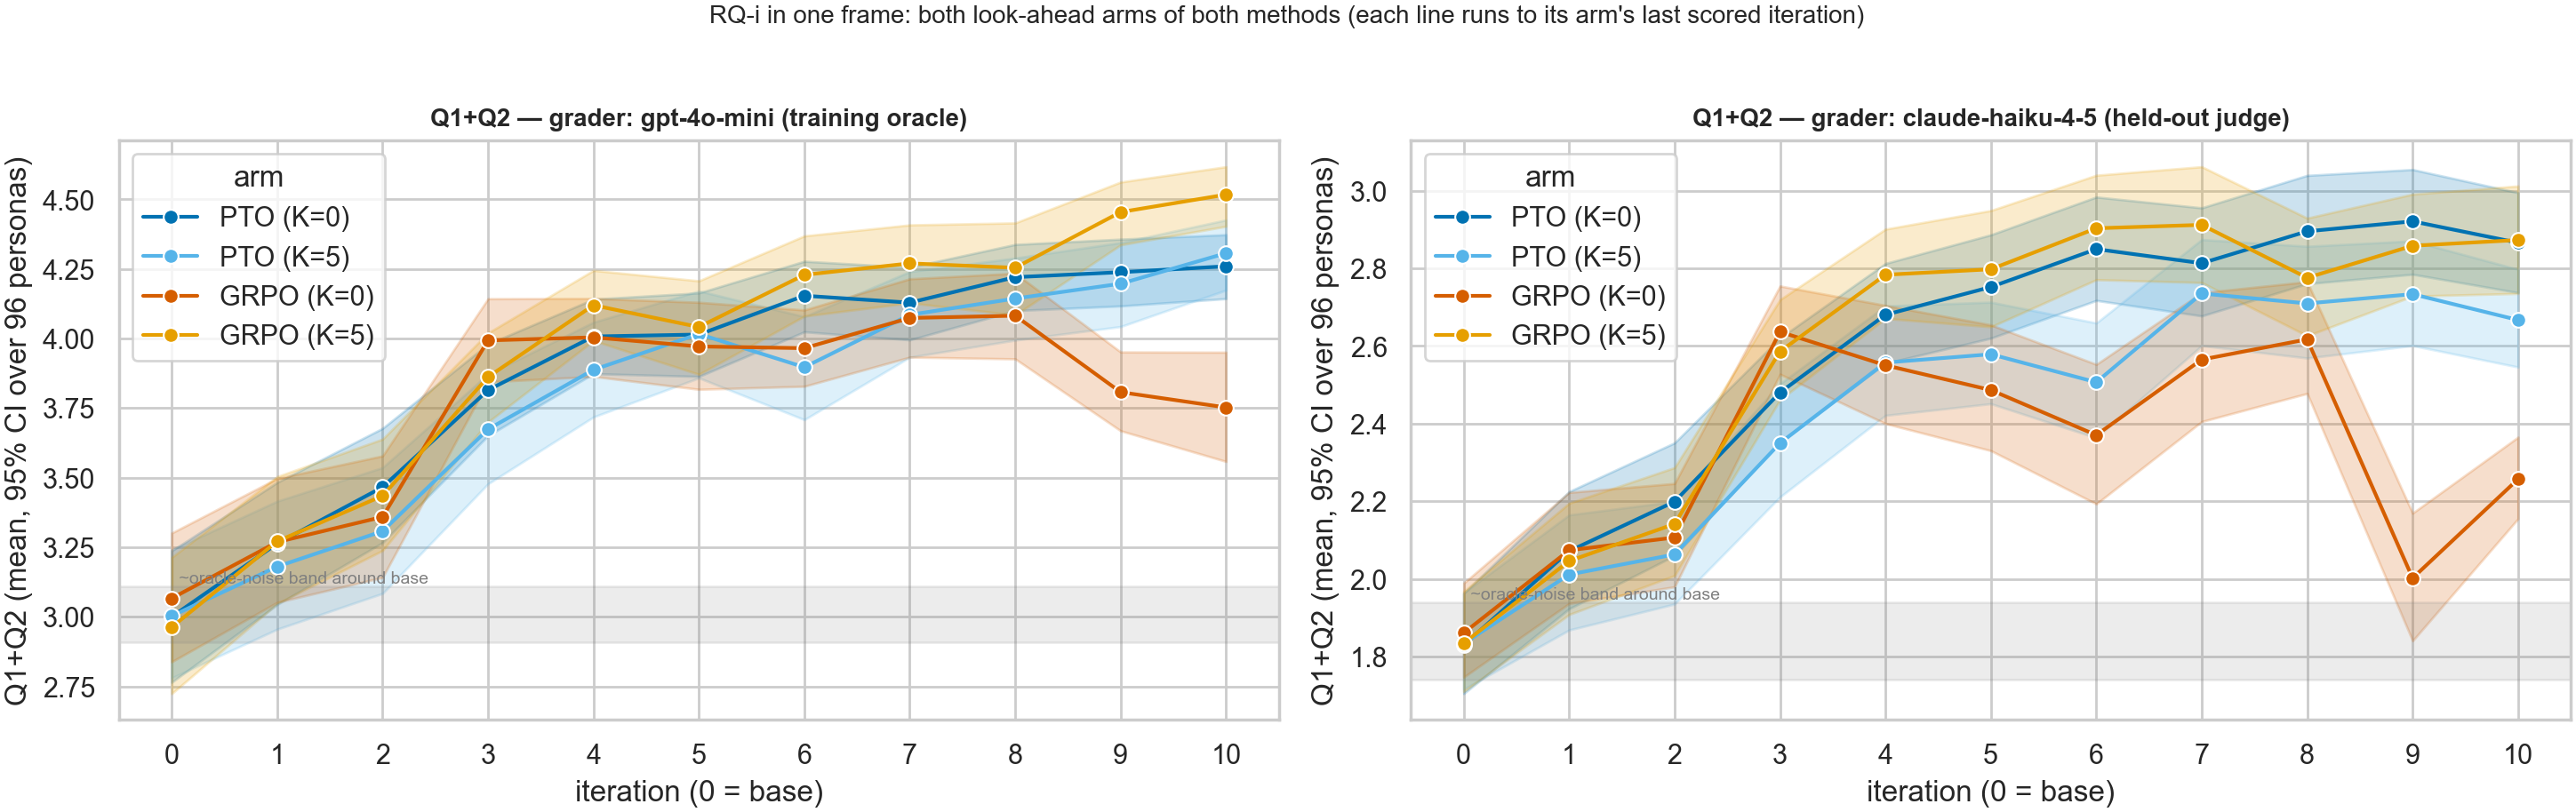
\includegraphics[width=0.98\textwidth]{figures/k_trajectory_Q1Q2.png}
\caption{All four arms in scores: \QQ\ by iteration (mean with 95\% CI over the 96 personas), one
panel per grader, both optimizers at both horizons. The two panels' $y$-axes are independent ---
the graders' levels are never comparable. The crossing structure is the paper's subject: the
\PTO\ arms dominate the middle of the run, and only \GRPO\ $\Kf$ ends above them.}
\label{fig:trajectory}
\end{figure*}

\subsection{By lever: look-ahead transforms GRPO and does not move PTO's outcomes}

Against each arm's own base on the rewarded rubric \QQ, under the training oracle: \GRPO's gain
goes from $+0.686$ ($\Kz$) to $+1.554$ ($\Kf$) --- the lever more than doubles it --- while
\PTO's goes from $+1.259$ to $+1.304$, statistically indistinguishable. The held-out judge agrees
on both: \GRPO\ $+0.396 \rightarrow +1.038$; \PTO\ $+1.036 \rightarrow +0.833$, a nominal
\emph{decline}. At the matched iteration-10 endpoint the within-optimizer $K$ contrast
(persona-paired, $n{=}96$) is, for \GRPO, $+0.765$ (\dz\,$0.905$) under the training oracle and
$+0.616$ (\dz\,$1.030$) held out --- significant on all eight instruments under both graders ---
and, for \PTO, $+0.047$ ($p_{\text{holm}}\,.70$) and $-0.199$ (\dz\,$-0.31$,
$p_{\text{holm}}\,.23$): null on the composite under both graders, with two held-out instruments
significantly \emph{worse} under $\Kf$ (Q2 $-0.363$, \dz\,$-0.65$; MITI $-0.203$, \dz\,$-0.49$).

The one place look-ahead helps \PTO\ in this regime is not an outcome score but a conduct one:
MI-inconsistent behaviour is significantly lower under $\Kf$ on \emph{both} graders ($-0.228$,
\dz\,$-0.71$ training oracle; $-0.245$, \dz\,$-0.66$ held out), and patient change talk is higher
under the held-out judge. \S\ref{sec:behaviour} returns to this: the lever's behavioural effect
is common to both optimizers even where its score effect is not.

\subsection{By optimizer: the sign flip}

The same numbers, cut the other way, are the headline
(Table~\ref{tab:flip}; full per-instrument endpoint grid in Appendix Table~\ref{tab:endpoints}).
At $\Kz$, \PTO\ beats \GRPO\ at the matched endpoint under both graders; at $\Kf$, \GRPO\ beats
\PTO\ under both graders. The interaction --- the difference-in-differences on the paired
per-persona contrasts --- is $0.718$ (\dz\,$0.793$, $p_{\text{holm}} < .001$) under the training
oracle and $0.815$ (\dz\,$0.972$) under the held-out judge, and is significant from iteration 4
onward. This is not a small moderation: the interaction's effect size is comparable to the
largest single-lever effects in the experiment.

\begin{table}[t]
\centering
\small
\setlength{\tabcolsep}{4pt}
\begin{tabular}{@{}llrrr@{}}
\toprule
Grader & Contrast (\PTO\ $-$ \GRPO) & $\Delta$ & \dz & $p_{\text{holm}}$\\
\midrule
\multirow{2}{*}{\primaryjudge}
 & at $\Kz$ & $+0.507$ & $0.729$ & $<.001$\\
 & at $\Kf$ & $-0.210$ & $-0.356$ & $.001$\\
\addlinespace
\multirow{2}{*}{\heldoutjudge}
 & at $\Kz$ & $+0.609$ & $1.265$ & $<.001$\\
 & at $\Kf$ & $-0.206$ & $-0.313$ & $.034$\\
\midrule
\multicolumn{2}{@{}l}{DiD, \primaryjudge} & $0.718$ & $0.793$ & $<.001$\\
\multicolumn{2}{@{}l}{DiD, \heldoutjudge} & $0.815$ & $0.972$ & $<.001$\\
\bottomrule
\end{tabular}
\caption{The sign flip on \QQ\ at the matched iteration-10 endpoint, persona-paired ($n{=}96$).
Positive means the preference-tree method scored higher. The difference-in-differences (DiD) is
the optimizer gap at $\Kz$ minus the gap at $\Kf$, computed on the paired per-persona
differences.}
\label{tab:flip}
\end{table}

\subsection{Every cell survives a second evaluation draw}

Each model state is scored on one 96-conversation sample with unseeded decoding, so before
leaning on the flip we re-drew the two winning endpoints --- 96 fresh conversations each from the
\GRPO-$\Kf$ and \PTO-$\Kz$ iteration-10 adapters, same personas, scored on all eight instruments
by both graders. The re-draws first establish a noise floor at \emph{trained} checkpoints: 36
same-policy contrasts (9 instruments $\times$ 2 graders $\times$ 2 states), none significant,
max $|\dz|\,0.216$. Substituting the re-draws into the headline contrasts changes nothing that
matters: the optimizer gap at $\Kz$ reads $+0.516$ / $+0.659$ (vs.\ $+0.507$ / $+0.609$
originally), at $\Kf$ $-0.155$ / $-0.227$ (vs.\ $-0.210$ / $-0.206$), and the \GRPO\ $K$ lever
$+0.709$ / $+0.637$ (vs.\ $+0.765$ / $+0.616$) --- same signs, same Holm significance, effect
sizes within $0.08$. A re-draw bounds evaluation noise only; there is still one training run per
arm (Limitations).
